%\documentclass[handout]{beamer}
\documentclass[public]{beamer}
\usepackage{econtexShortcuts}
\usepackage{ifthen}
\usepackage{verbatim}

\usetheme{Madrid}
\definecolor{orange}{HTML}{FF7F00}\hypersetup{colorlinks,linkcolor=,urlcolor=orange}

% Redefine footer from
% http://tex.stackexchange.com/questions/83048/change-the-contents-of-footline-in-a-beamer-presentation
\setbeamertemplate{footline}
{
  \leavevmode%
  \hbox{%
  \begin{beamercolorbox}[wd=.333333\paperwidth,ht=2.25ex,dp=1ex,center]{author in head/foot}%
    \usebeamerfont{author in head/foot}\insertsection
  \end{beamercolorbox}%
  \begin{beamercolorbox}[wd=.333333\paperwidth,ht=2.25ex,dp=1ex,center]{title in head/foot}%
    \usebeamerfont{title in head/foot}\insertsubsection
  \end{beamercolorbox}%
  \begin{beamercolorbox}[wd=.333333\paperwidth,ht=2.25ex,dp=1ex,right]{date in head/foot}%
    \usebeamerfont{date in head/foot}\insertshortdate{}\hspace*{2em}
    \insertframenumber{} / \inserttotalframenumber\hspace*{2ex} 
  \end{beamercolorbox}}%
  \vskip0pt%
}
\makeatother

\providecommand{\ARK}{\href{http://github.com/econ-ark}{github.com/econ-ark}}

\providecommand{\CDC}{\texttt{CDC}}
\providecommand{\NMP}{\texttt{NMP}}
\providecommand{\MNW}{\texttt{MNW}}
\providecommand{\DCL}{\texttt{DCL}}
\providecommand{\JXY}{\texttt{JXY}}
\providecommand{\ABK}{\texttt{ABK}}

\provideboolean{CESifo}
\setboolean{CESifo}{true}
\setboolean{CESifo}{false}
\providecommand{\CESifoYN}{\ifthenelse{\boolean{CESifo}}}

\provideboolean{NBERMtoM}
\setboolean{NBERMtoM}{true}
\setboolean{NBERMtoM}{false}
\providecommand{\NBERMtoMYN}{\ifthenelse{\boolean{NBERMtoM}}}

\provideboolean{GMU}
\setboolean{GMU}{true}
\providecommand{\GMUYN}{\ifthenelse{\boolean{GMU}}}
 
\beamerdefaultoverlayspecification{<+->}
 % Switch allow external script to determine whether compiling this generates print version or handout version



\usepackage{natbib}
\begin{document}
\title[\ARK]{Introducing  the Computational Economics \\ ``Algorithmic Repository and toolKit'' \\
\href{http://github.com/econ-ark}{github.com/econ-ark}}

\CESifoYN{
\author[Chris Carroll, Matthew White]{Presentation by Chris Carroll and Matthew White at  \\ {CESifo Conference, Venice}}
\date{June 13, 2017}
}{}

\NBERMtoMYN{
\author[Chris Carroll, Matthew White]{Presentation by Chris Carroll and Matthew White at  \\ NBER Summer Institute ``Micro to Macro'' Working Group}
\date{July 17, 2017}
}{}

\GMUYN{
\author[Chris Carroll, Jackie Kazil]{Presentation by Chris Carroll and Jackie Kazil at  \\ George Mason University Department of Computational Social Sciences}
\date{March 30, 2018}
}{}

\begin{frame}
  \titlepage
\end{frame}

\section{Who, What, Where, When, Why}
\GMUYN{}{
\subsection{What}

\begin{frame}\frametitle{Do for HA Macro What DYNARE Did for RA}

\pause Provide state-of-the-art set of tools for:
\begin{enumerate} \pause
\item Solving dynamic stochastic optimization problems
\begin{itemize}
\item `Hard' Bellman problems with uncertainty, `kinks,' nonconvexities
\end{itemize}
\item Simulate behavior of populations of agents
  \GMUYN{
  \bi
\item Whether or not they are solving DSOP
  \ei}{}
\item Finding equilibria for markets/economies populated by such agents
\end{enumerate}
\end{frame}
}

\GMUYN{\begin{comment}}{}
\begin{frame}
\frametitle{What Is It Good For?}

\begin{itemize}
\item Heterogeneous Agent Macro Models
\begin{itemize}
\item Original name: {\bf H}eterogeneous {\bf A}gent {\bf R}esources and tool{\bf K}it
\item HARK!
\end{itemize}
\item Structural Micro Models (e.g., labor, health)
\item IO models with equilibrim between consumer agents and firm agents
  \CESifoYN{}{
\item {\bf N}ot {\bf O}nly {\bf A}bout {\bf H}eterogeneous {\bf s}tuff ... 
\item ... {\bf A}lgorithmic {\bf R}esources and tool{\bf K}it 
\item :-)
\begin{itemize}
\item Unlike Noah's, our ARK can hold more than two of each kind!
\item Ultimate goal: Get examples on the ARK of all types of animal (model)
\end{itemize}

\end{itemize}
\end{frame}


\subsection{Why}
\begin{frame}\frametitle{Why Have We Created It?}

Micro Structural Modeling 2017 $\approx$ Econometrics circa 1970 
\bi
\item Lots of theoretical results
\item Actual applications must be hand crafted at enormous cost
  \bi
\item 1970 econometrics: Write your own matrix inversion package!
  \item 2017 structural: Write your own numerical convergence alogrithms
  \ei
\item Lots of reinventing of the wheel
  \item Progress is very slow
  \ei

\end{frame}

\GMUYN{\end{comment}}{}

\begin{frame}\frametitle{Goals}

  Make it {\it much} easier:   \pause 
  \bi
\item To get started doing structural Heterogeneous Agent modeling
\item To teach (with hands-on, problem-set-assignable exercises)
\item To {\it compare} models to each other
\item To add new capabilities
\item To mix-and-match components/modules/agent types
  \ei

\pause Remove the excuse `Structural model was not worth the effort'
  
\end{frame}

\subsection{How}
\GMUYN{\begin{comment}}{}
\begin{frame}\frametitle{How Do We Expect To Do This?}

  
\bi  
\item Has been done already in many other scientific/technical fields
\bi
\item AstroPy
\item Statistics: `R' and the Journal of Statistical Software
  \item Many open-source resources in other sci/tech fields 
    \ei
    \ei

    \medskip\medskip
  }

\end{frame}
\GMUYN{\end{comment}}{}

\GMUYN{}{
\begin{frame}\frametitle{Now: HA Structural Modeling Is Alchemy Not Chemistry}

... for outsiders: \pause Magic (done by mages!) 

  \bi \pause
\item This is unfair: Alchemists {\it tried} to hide their methods 
  \ei
  
\pause  Need to make it `normal science': \pause
  \bi
\item Transparent, reproducible
  \item {\it easy} (not hard) to `stand on the shoulder of giants'
  \ei
\end{frame}
}

\begin{frame}\frametitle{Github=Gutenberg}
\pause Suite of powerful modern tools developed by software engineers: \pause    
    \bi
  \item Almost-Automatic Integrated Documentation
  \item Robust Built-In Testing 
  \item Continuous Integration
  \item Version Control
  \item Object-Oriented Programming (Python!)
  \item Integrated Development Environments
  \item Apache License 
  \item ...
    \ei
    \medskip

  \end{frame}

  

\begin{frame}\frametitle{Will We Succeed?}  
\pause A {\it lot} of enthusiasm from deep-pocketed policy institutions     \pause

\bi \item CFPB - Lion's Share of the Credit For Getting Here
  \bi
\item Hired CDC As Chief Economist
  \bi
  \item On Specific Premise that Toolkit Would Be Priority
    \ei
    \item Hired MNW (leave of absence from UDel) To Create It 
  \ei
  \ei
  
    \bi
  \item Central Banks
    \bi \item So far: Fed (Board and Banks), ECB, BoE, RBA, RBNZ
    \ei 
  \item IMF
  \item OFR
    \ei
    
\end{frame}

\begin{frame}\frametitle{Just Received Big Grant from Alfred P. Sloan Foundation!}  

  Three Years \pause
  \bi
  \item Hire Programmers, RA's, Open Source Project Managers, etc etc
  \ei
  
\end{frame}

\GMUYN{}{
\section{An Example}

\begin{frame}{Application: From All-Day Fed Workshop ...}

Should we take `uncertainty' seriously as explanation for this:

\begin{center}
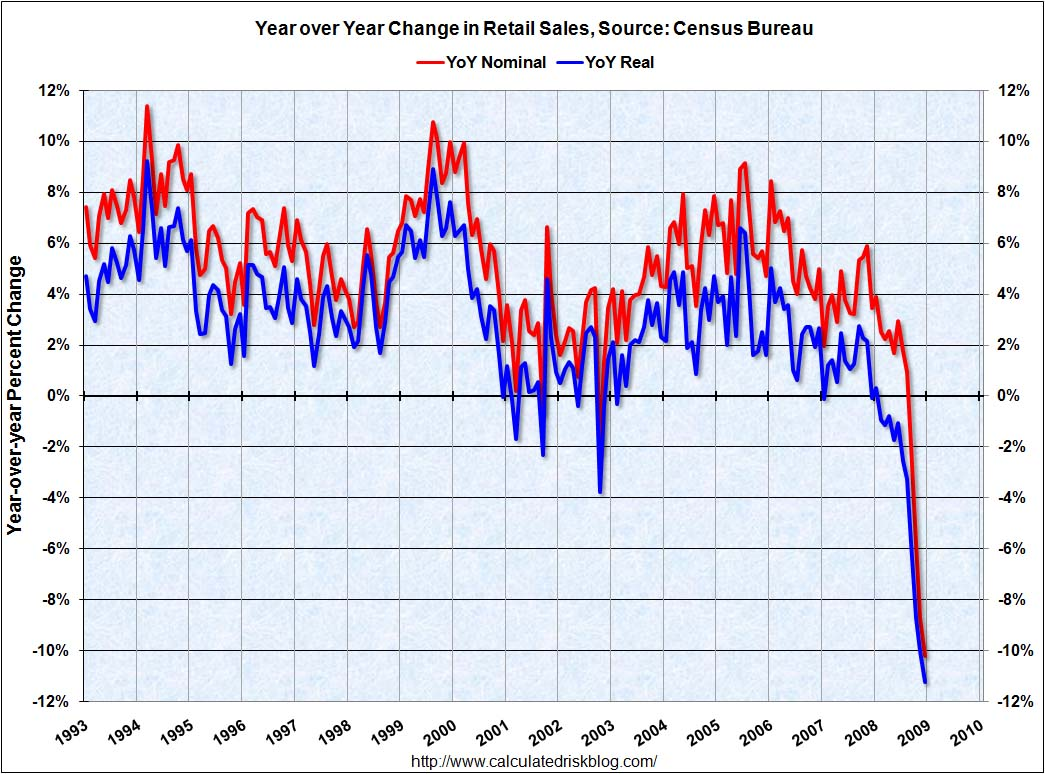
\includegraphics[width=3in]{/Volumes/Data/Code/ARK/PARKive/pri/PARK-make/Intro-To-ARK/ForEconomists/Figures/Retail-Sales-Collapse.jpg}
\end{center}
  
\end{frame}

\begin{frame}{From All-Day Fed Workshop ...}

  Of course `uncertainty' is fashionable right now
  \begin{itemize} \pause
    \item Susanto Basu
  \item Nick Bloom
    \item Larry Christiano (!)
  \item Steve Davis
  \item Ulrike Malmendier
    \item ...
    \end{itemize}

\pause    ... because $C$ collapse vastly exceeds what can be explained by traditional macro variables (wealth, credit supply, ...)
    
\end{frame}

\begin{frame}{From All-Day Fed Workshop ...}

  It's a Quantitative Theory question:
  \bi
\item {\it How Big} would increase in $\sigma_{\psi}^{2}$ need to be to generate {\it entire} observed $C$ collapse?
  \ei

  \pause
  \bi
  \item If answer is absurd, maybe we have to look elsewhere
  \ei
  
\end{frame}

\begin{frame}{From All-Day Fed Workshop ...}

  Exercise: 
  
  \bi
\item Take \cite{cstwMPC} model in ARK
  \item Traditional calibration (from Carroll (1992)!) so hands are tied
  \item Ask `how much of an increase in $\sigma^{2}_{\psi}$ would explain entire $C$ collapse'?
  \ei

\pause ... over to MNW!  
  
\end{frame}
}
\beamerdefaultoverlayspecification{<*>}

\begin{frame}[t,allowframebreaks]
\frametitle{References}
\tiny 
\input econtexBibMake
\end{frame}
\pagebreak

\end{document}

\subsection{How}
\GMUYN{\begin{comment}}{}
\begin{frame}\frametitle{What Makes Us Think This is Feasible?}

\bi  
\item Has been done already in many other scientific/technical fields
\bi
\item AstroPy
\item Statistics: `R' and the Journal of Statistical Software
  \item Many open-source resources in other sci/tech fields 
    \ei
    \ei

    \medskip\medskip
  
  \end{frame}
    \GMUYN{\end{comment}}{}

\subsection{Where}
\begin{frame}
\frametitle{Where Is It?}

\begin{center}
{\ARK} is the project's home
\end{center}

\begin{enumerate}
  \GMUYN{}{
\item Get a GitHub account.  Then, options to access are
\begin{itemize}
\item Install GitHub Desktop App
\item Install `git' command-line tool (if you're hard-core)
\end{itemize}
}
\item \texttt{{\ARK}/HARK} is a ``public repo'' 
\begin{itemize}
\item Contains all existing code
\end{itemize}
\CESifoYN{}{
\item \texttt{{\ARK}/HARK/Documentation/NARK.pdf}
\begin{itemize}
\item Describes variable naming conventions for easy workflow: 
\item LaTeX object definitions correspond to HARK definitions 
\end{itemize}
\item Similar structure will be used for future contributions
\begin{itemize}
\item {\bf A}gent {\bf A}rchive {\bf R}epository {\bf D}eposit {\bf V}ehicle for ARK?
\end{itemize}
}{}
\item Instructions for cloning are in the README.txt
\item You get the whole codebase under the Apache license 
\begin{itemize}
\item Basically, no limitations on use
\item But, please credit us, and participate in discussions
\end{itemize}
\end{enumerate}

\end{frame}

\subsection{Who}
\GMUYN{}{
\begin{frame}
\frametitle{Who Has Produced It?}

\begin{footnotesize}
\begin{center}

\begin{tabular}{lll}
Name & TLA & Affiliation % & Contact
\\ \hline \hline {\it Christopher D Carroll} & \texttt{{\CDC}} & JHU, CFPB % & \href{mailto:ccarroll@llorracc.org}{ccarroll@llorracc.org}
\\ {\it David C Low} & \texttt{{\DCL}} & CFPB % & \href{mailto:ccarroll@llorracc.org}{ccarroll@llorracc.org}
\\ {\it Nathan M Palmer} & \texttt{{\NMP}} & OFR % & \href{malito:nathan.m.palmer@gmail.com}{nathan.m.palmer@gmail.com}
\\ {\it Matthew N White} & \texttt{{\MNW}} & UDel, CFPB % & \href{mailto:mnwhite@gmail.com}{mnwhite@gmail.com}
\\ \hline {\it Alex Kaufman} & \texttt{{\ABK}} & CFPB $\rightarrow$ ? (Timbuktu?)  %& \href{mailto:alexander.kaufman@cfpb.gov}{No Fixed Address; Expected: Alcatraz}
\\ {\it Jiaxiong Yao} & \texttt{JXY} & JHU $\rightarrow$ IMF  %& \href{mailto:alexander.kaufman@cfpb.gov}{No Fixed Address; Expected: Alcatraz}
\end{tabular}
\end{center}


Nothing herein may be interpreted as reflecing opinions of 
\begin{center}
\begin{tabular}{rcl}
 CFPB & - & United States Consumer Financial Protection Bureau
\\ JHU & - & Johns Hopkins University
\\ IMF & - & International Monetary Fund
\\ OFR & - & Office of Financial Research, U.S.\ Treasury
\\ UDel & - & University of Delaware
\end{tabular}

\end{center}


\end{footnotesize}
\end{frame}
}

\begin{frame}
\frametitle{Major credit to CFPB }

\begin{itemize}
\item Hired {\CDC} as Chief Economist with this as a key priority
\item Hired {\NMP} as intern to get started
\item Hired {\MNW} as Visiting Scholar to work on it
\item Hired {\DCL} as new economist last year
\item Hired {\ABK} as RA
\end{itemize}
\end{frame}


\begin{frame}
\frametitle{Organization Going Forward}

Standard Github tools, esp:
\begin{itemize}
\item Issue Tracker: If You See Something, Say Something
\end{itemize}
\begin{center}
{\bf Topic Czars}

\begin{itemize}
\item Gatekeeper for Contributions
\item Responsible for Setting Out Tests A Module Should Pass
\begin{itemize}
\item e.g.\ Special Cases With Analytical Solutions
\item Metrics for ``closeness'' to ``true'' solution
\end{itemize}
\end{itemize}

\pause 
\begin{tabular}{lll}
Name & Topic & Affiliation
\\ \hline  Serguei Maliar & Interpolation & Stanford %& \href{mailto:ccarroll@llorracc.org}{ccarroll@llorracc.org}
\\ Lilia Maliar & Interpolation & Stanford % & \href{}{mailto:ccarroll@llorracc.org}
\\  \multicolumn{3}{c}{{\it We're Seeking Volunteers for Czars}}
\end{tabular}
\end{center}

\pause
\begin{tabular}{rcl}
\hline \href{mailto:info@econ-ark.org}{info@econ-ark.org} & - & General Purpose Questions
\\ \href{mailto:czars@econ-ark.org}{czars@econ-ark.org} & - & Volunteer to be a Czar
\\ \href{mailto:ideas@econ-ark.org}{ideas@econ-ark.org} & - & Ideas for Improvement
\end{tabular}


\end{frame}

\subsection{When}

\begin{frame}
\frametitle{Timeline}

\begin{center}
\begin{tabular}{rll}
When & What & Lessons
\\ \hline 2006-2013 & \href{http://econ.jhu.edu/people/ccarroll/SolvingMicroDSOPs}{SolvingMicroDSOPs} & Surprisingly popular
\\ 2014-12 & \href{}{IMF-CFPB Workshop} & Lots of enthusiasm
\\ 2015-12 & \href{}{CFPB-IMF Workshop} & Not HARK, ARK!  
\\ & & Testing, Replication, Feedback
\\ 2016-06 & Hello! & None yet ...
\end{tabular}
\end{center}

\begin{itemize}
\item The version at \href{github.com/econ-ark}{http://github.com/econ-ark}  is our ``public beta''
\item So far as we know, everything works
\item First non-beta: Built-in tests for {\it everything}
\begin{itemize}
\item Aim: This year
\end{itemize}
\end{itemize}

\end{frame}

\subsection{Why?}
\begin{frame}
\frametitle{Why Are Policy Institutions So Interested?}

Participation: CFPB, OFR, IMF 

Interest From: FRB, ECB, BLS

\begin{itemize}
\item Policymaking = Applied Theory.  Options:
\begin{enumerate}
\item Informal, intuitive, ``wetware'' theory 
\item Formal, structural, ``software'' theory 
\end{enumerate}
\end{itemize}

\end{frame}

\begin{frame}
\frametitle{LATE is Antedeluvian}

`Local Average Treatment Effects' results are 
\begin{itemize}
  \item {\bf N}ot {\bf E}ven {\bf V}ery {\bf E}mpirically {\bf R}elevant ...
  \item UNLESS used to estimate `structural' parameters
\item Because the important question is
\begin{itemize}
\item What does world look like {\it non-locally} ...
\item ... = {\it after} the policy change
\item and maybe not even just ``on average''
\begin{itemize}
\item because distributional/targeted impact may be whole point
\end{itemize}
\end{itemize}

\end{itemize}

\end{frame}

\begin{frame}
\frametitle{Welfare Analysis With Heterogeneity}

Sensible cost-benefit analysis requires:
\begin{itemize}
\item Estimates of distribution of heterogeneous outcomes 
\item Utility or other weighting of those outcomes
\item $\rightarrow$ Structure
\end{itemize}

\end{frame}

\subsection{How}

\begin{frame}
\frametitle{{\it The Invention of Science} by David Wootton}

Wrong explanations for the Scientific Revolution: \pause 
\begin{itemize}
\item Invention of `the experiment'
\item Invention of the printing press
\item ... 
\end{itemize}
\medskip\medskip

\pause 
Right explanation:
\begin{itemize}
\item Creation of community of scholars
\item ... whose methods and results were `open source'
\item ... who critcized and improved and debugged each other
\end{itemize}

\medskip
\pause
Alchemy $\rightarrow$ Chemistry

\medskip
\pause 
17th and 18th century version of \href{http://github.com}{github.com}!

\end{frame}

\begin{frame}
\frametitle{Economists are People Too ...}

\begin{itemize}
\item We are {\it way} behind many scientific fields in `open source' code
\item Surveys/Experiments: Economics students are more `selfish.'
\item Options: \pause
\begin{enumerate}
\item `selfish' people study economics
\item Studying economics makes you selfish!
\item Economics students are just more honest
\end{enumerate}
\end{itemize}

\pause I prefer (3)!

\end{frame}

\begin{frame}
\frametitle{Lessons Learned from Other Fields About What Works}

\begin{itemize}
\item Not taking the dewy-eyed view: ``Build it and they will come''
\item Emprical fact: Many other open source communities have succeeded
\item Economists can't be {\it that} different ...
\end{itemize}

\end{frame}

\begin{frame}
\frametitle{In Addition to Usual Github Tools}

\begin{itemize}
\item Czars for specific topics
\item Bounties for Best Solution of Specific Problems
\item Time-Stamped Public Mechanism for Staking a Claim to New Idea
\item Stack-Exchange-Like Q\&A Forum
\item Mechanism for Easy Creation of Grad Student Problem Sets
\item Tool for Grad Student Replication Exercises
\item Eventually, a Journal?
\item ... Your Ideas?  \href{mailto:ideas@econ-ark.org}{ideas@econ-ark.org}
\end{itemize}

\end{frame}

\begin{frame}
\frametitle{Join our (Scientific) Revolution!}

\providecommand{\subscribe}{\href{mailto:subscribe@econ-ark.org}{subscribe@econ-ark.org}}
\providecommand{\letmehelpwith}{\href{mailto:letmehelpwith@econ-ark.org}{letmehelpwith@econ-ark.org}}
Options:
\begin{itemize}
\item \subscribe
\begin{itemize}
\item Add me to the newsletter/mailing list
\end{itemize}
\item {\it Read the docs and slides} and absorb what exists now.  Options:
\begin{enumerate}
\item Add an `issue' that you want to tackle on \ARK
\item \letmehelpwith
\begin{enumerate}
\item Define some area that you'd like to contribute to
\item email us at this address outlining what you propose to do
\item We'll reply with some suggestions
\end{enumerate}
\end{enumerate}
\end{itemize}

\end{frame}

\end{document}

